\section{Vorgehen}
In diesem Kapitel wird das Vorgehen beschrieben, wie die Arbeit geplant und realisiert wurde.

\subsection{Arbeitsmethodik}
Da die Arbeit nur von einem Autor umgesetzt wurde, musste bezüglich Arbeitsmethodik nur wenig definiert und koordiniert werden.

Um zu starten, hat dem Autor geholfen, dass der Experte \prof\space bereits anfangs Sommer (16. Juli) einen ersten Besprechungstermin angesetzt hat. Um eine Diskussionsbasis für diesen Termin zu haben, musste sich der Autor ernsthaft mit der Semesterarbeit auseinandersetzen. Dazu hat er aus einer BFH Vorlage \footnote{Herzlichen Dank an Andreas Habegger und Lukas Studer fürs Bereitstellen der \href{https://gitlab.ti.bfh.ch/latex-utils/tpl_latex-thesis}{Vorlage}} ein Gerüst der Arbeit erstellt und stichwortartig abgefüllt. Nach gründlicher Diskussion mit dem Experten wurde dieses Gerüst etwas angepasst und diente von da an als Basis für die Arbeit; wo sich die Kapitel zunehmend von losen Notizen zum finalen Zustand festigten.

Um die Übersicht nicht zu verlieren, wurde beschlossen, nach Kanban zu arbeiten, respektive ein Kanban Board zu verwenden. Weil für die Arbeit sowieso Repository auf \emph{github.com}\footnote{\href{https://github.com/bfh-semesterarbeit/spot-geoprocessing/projects/1}{Projekt auf github.com}} angelegt wurde, konnte dort auch gleich ein Kanban erstellt werden. Das Kanban Board wurde vor allem auch dafür genutzt, fortlaufend neue kleine Aufgaben aufzulisten und darauf zu achten, die Menge der angefangenen Arbeit zu begrenzen.

Dadurch konnte im Alltag (wenn gerade etwas Zeit zur Verfügung stand) eine solche Aufgabe genommen und erledigt werden. Es wurde nicht strikte nach Kanban gearbeitet, aber einige Prinzipien daraus wurden verwendet. Zum Beispiel wurde das erste Grundprinzip angewendet \textit{"Beginne mit dem, was du gerade tust:
In diesem Grundprinzip stecken zwei Dinge. Indem man mit dem beginnt, was man gerade tut, beendet man die aktuelle Arbeit, bevor etwas Neues begonnen wird. Genauso ist hier aber auch die Aussage enthalten, dass Kanban einfach eingeführt werden kann."}\cite{kanban2010}. Eine Momentaufnahme des Kanbans befindet sich im Anhang \ref{appendix:kanban}.

\subsection{Projektplan}\label{chap:projektplan}
Um den übergeordneten Rahmen der Arbeit nicht aus dem Fokus zu verlieren und um sich bewusst zu machen, wieviel Zeit generell bis zur Abgabe zur Verfügung steht, war es hilfreich, einen Projektplan mit Meilensteinen konsultieren zu können. Durch die Berner Fachhochschule waren die grundlegenden Meilensteine bereits vorgegeben. Der Projektplan befindet sich im Anhang \ref{appendix:projektplan}.

\subsection{Vorarbeiten}
\subsubsection{AWS Account}
\begin{itemize}
	\item Fit werden mit AWS
\end{itemize}

\subsubsection{AWS Spot Instances}
\begin{itemize}
	\item Herausfinden wie mit AWS Spot Instanzen gearbeitet werden kann
\end{itemize}
\begin{figure}[H]
	\centering
	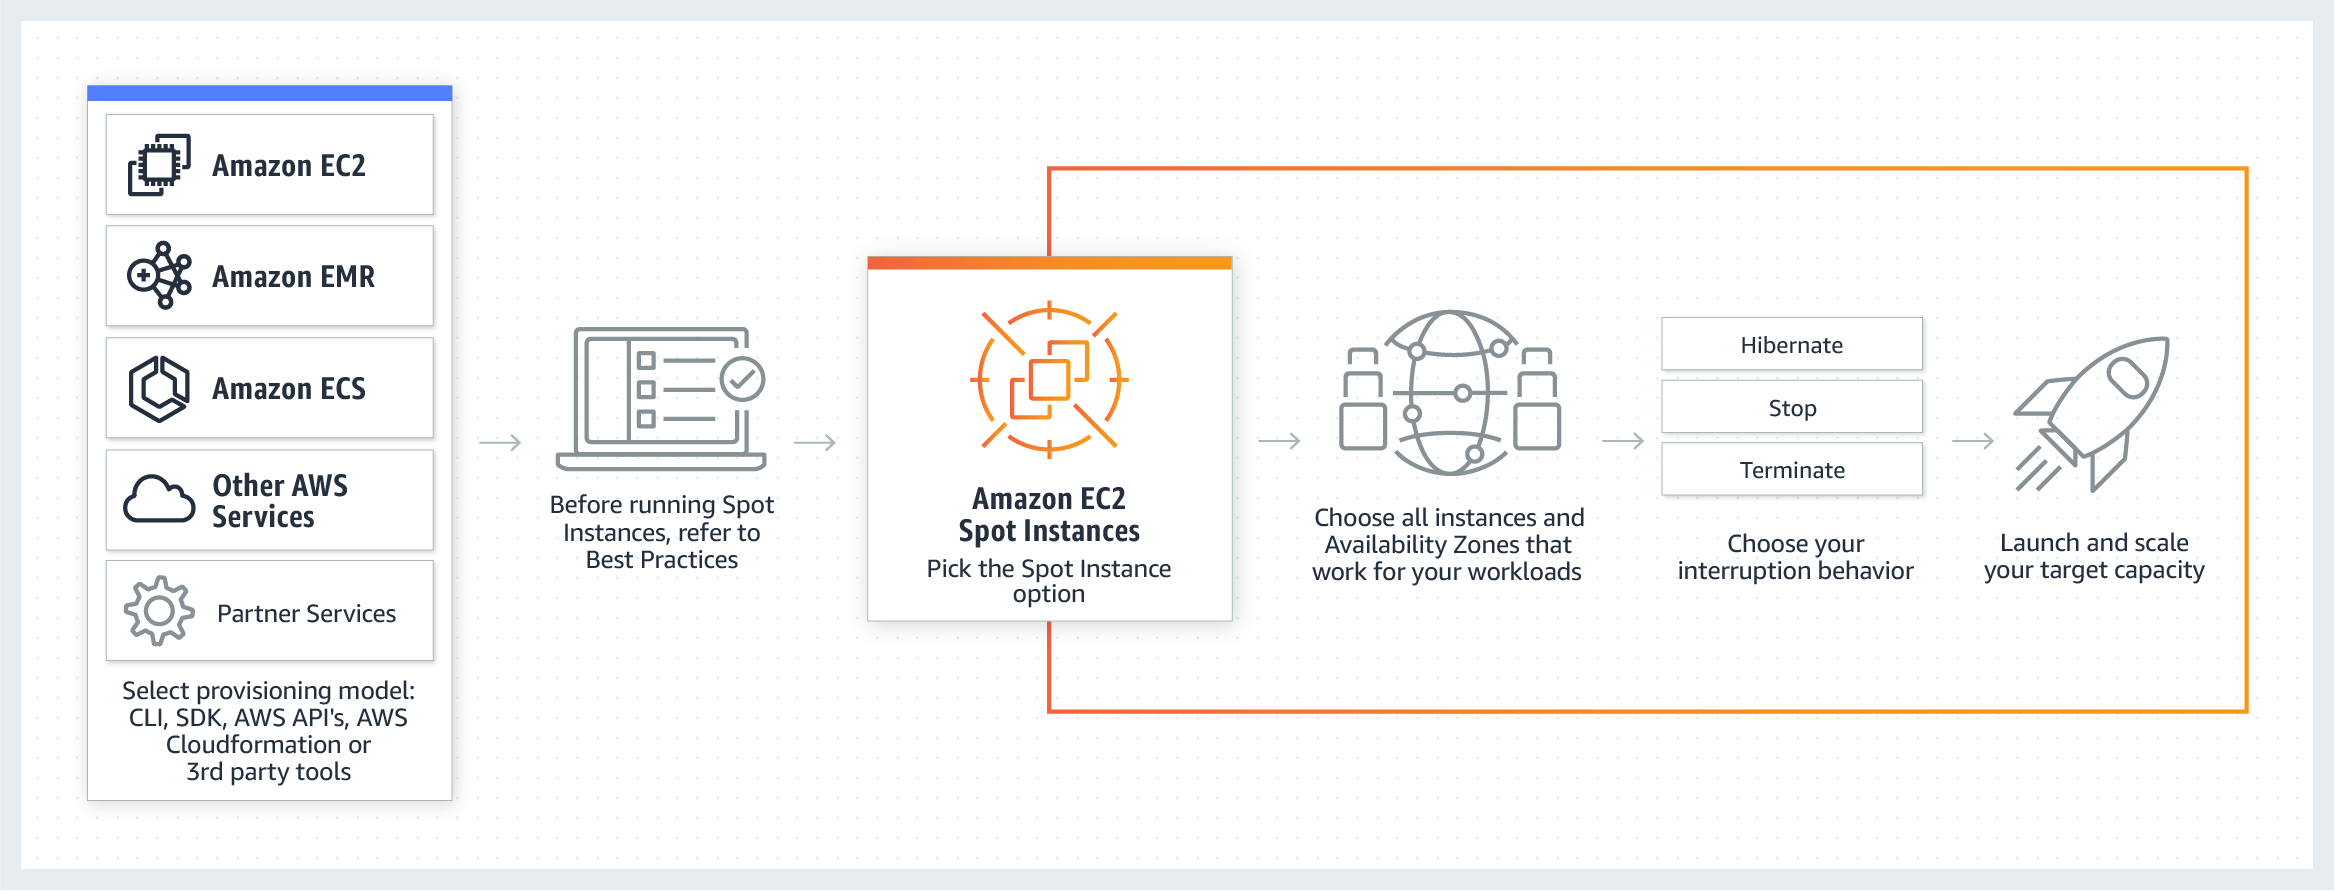
\includegraphics[width=.6\textwidth]{spot}
	\caption{AWS Architektur Spot\cite{AmazonAWSSpot:1}}
	\label{fig:AWS Architektur Spot}
\end{figure}

\subsubsection{Kubernetes testing}
\begin{itemize}
	\item Anfangs mit Minicube
	\item Eigenem AWS account
\end{itemize}
